\begingroup
\chapter*{Introduction\markboth{Introduction}{}}
\addcontentsline{toc}{chapter}{Introduction}
\renewcommand\thefigure{I.\arabic{figure}}

Noise is a major issue in our modern societies, ranging from everyday life inconveniences, work comfort problems to an actual pollution problem in severly affected areas. Sources of noise can be diverse; in urban environments, concerns are mostly on population and traffic noise. From industrial origins, noise can be of several consequences, causing not only risks to the workers and the neighbouring populations, but also structural hazard to installations. Generally, motorized transport is a major issue in all environments, including aircraft, public transportation, roads, commercial vessel traffic, etc. 

Although sound intensity can be measured objectively, the impact of noise on individuals is in part shaped by social and cultural context. Studies show that expected behaviours norms and customs strongly influence reported annoyance \cite{fields1993}, with comparative surveys revealing clear cross-cultural differences. More recent work has linked collectivistic cultural norms to systematically higher everyday noise exposure \cite{benitez-barrera2023, ramirez-esparza2024}.

The European Environment Agency estimated in 2021 that 1 in 5 European resident are exposed to unhealthy levels of noise, which mostly originates from traffic noise. These noise exposures can have a strong impact on health \cite{basner2014} favoring impaired circadian rythm, oxidative stress and cardiovascular dysfunction \cite{munzel2018}, as well as psychological consequences like anxiety and depression \cite{hahad2025}. Moreover, anthropic noise pollution also affects biodiversity at large, causing stress, behaviour changes, and masking sensory perception~\cite{sordello2020}. Marine traffic was shown to generate stress on marine mammals and modify their behaviour by provoking area avoidance and vocalization disruption \cite{erbe2019}.\\

The emergence of all these noise sources comes with the need to mitigate them up to our current capabilities. The latter is able to evolve thanks to research on noise barriers and acoustic insulation systems. Various acoustic insulation strategies have been applied throughout the ages. Dating back to 4th century BC, acoustic jars were used to improve the room acoustics in Greek and Roman theatres as well as in the Middle Ages in Western Europe in churches \cite{valiere2013}. These resonators are thought to be capable of reducing reverberation time in buildings, covering a frequency range matching that of human spoken voice. As another example, a famous roman amphitheater was shown to have a seat row disposition able to improve intelligibility of speeches from the stage \cite{declercq2007}. 

Contemporary to these antique devices, porous and fibrous materials have been traditionally used to absorb sound in the last century \cite{allard2009, bruneau2006, auriault2002, liu2014porous, bourbie1986acoustique, coussy2011mechanics}. Largely used in the industry, they are efficient at frequencies starting close to the quarter wavelength resonance frequency of the layer and have been extensively analyzed in the literature \cite{lafarge1993propag, lafarge1993, lafarge1997, duclos2006multiple, brouard1995general}. They can be found in natural occurences or engineered and cover very large use cases of acoustic insulation such as industry, transport, aerospace, concert halls and many others. The picture of a porous material is shown in Fig.~\ref{fig:porous_layers}a. \comment{(utile ?)}\\ 

\begin{figure}[htpb]
    \centering
    % a voir ce qui est pertinent de mettre dans cette figure
    \caption{a) Image de la microstructure d'un poreux b) Coefficient de réflexion et absorption d'une couche rigid-backed d'un PEM avec un schéma. c) Coefficient de réflexion, transmission et absorption d'une couche avec transmission d'un PEM avec un schéma. }
    \label{fig:porous_layers}
\end{figure}

\clearpage
\section*{State of art\markboth{Introduction}{State of art}}
\addcontentsline{toc}{section}{State of art}

\subsection*{Overview of Acoustic Metamaterials}
{\phantomsection \addcontentsline{toc}{subsection}{Overview of Acoustic Metamaterials}}
In more recent years, the emergence of more complex engineered structures has disrupted the landscape of acoustic absorbers. Metamaterials are composite structures designed to exhibit physical effective properties that go beyond the capability of the sole material that composes the bulk. They can be created by a lot of various means, including engineered microstructure, a gradial evolution of the material properties, or repeating patterns or scatterers implemented in one or several directions in space and embedded in a host material as shown for various dimensions in Fig.~\ref{fig:periodic_fig}. Compared to homogeneous layers, they generally lead to more complex structures, and are able to achieve enhanced effects. Usually allowing for a tunable response, these structures offer great flexibility and open new perspectives in material design. Therefore, they have sparked interest in various disciplines, such as photonics and optics \cite{russell2003}. They can be used to design antennas and absorber for electromagnetic waves, seismic protection devices among others. In acoustic, they allow for various applications such as absorption, filtering, diffusion or cloaking.

Seminal works have been done on the study of the use of lattice arrangements or crystals and have been applied to wave control application. Photonic crystals are used to achieve the control of light and electromagnetic waves \cite{yablonovitch1987}. Phononic crystals have been developed for the control of elastic and acoustic waves as the periodic distribution of scatterers in a solid host medium \cite{sigalas1992}. In the case where the host medium is constituted by a fluid, these structures are called sonic crystals \cite{martinez-sala1995}. These structures are often studied through their band structure (also called dispersion diagram when used to study non-periodic geometries). These diagram represents the wavenumber in a given direction against the frequency, thus informing on the evolution of the wave velocities in the structure and thus the dispersion. These aspects will be addressed in the subsequent chapter, especially regarding the background theory and the available numerical tools to compute them.

\begin{figure}[htpb]
    \centering
    
\includegraphics[width=.8\textwidth]{1to3D_schema.png}
    \caption{Periodic cells in 1, 2 and 3D. Image taken from Ref.~\cite{jimenez2021}}
    \label{fig:periodic_fig}
\end{figure}

In the remaining of the literature overview, focus will be centered around metamaterials that involve mostly periodicity in only one direction. These acoustic metamaterials solutions can be divided into two main categories: the first concerns the so-called \emph{reflection problem} where the case study is that of an incoming wave on some sample or panel which has a rigid-backing at the end. There, the consideration is focused on mitigating the reflected wave and acheving important acoustic absorption. The other case is that of a \emph{transmission problem} where the incoming wave is able to transmit through the sample. In this case and depending on the application, either or both reflection and transmission are sought to be mitigated. The symmetry of the structure is of importance in this case. 

Structured materials that tackle the reflection problem can involve many various strategies. The combination of a perforated plate and coiled-up channels is able to achieve large broadband absorption underwater\cite{zhou2023}. Micro-perforated plate can also be used to achieve interesting absorption properties for airborne acoustics\cite{prasetiyo2021}. Materials structured from resonant building blocks with resonance frequencies in the sub-wavelength regime i.e., for frequencies which wavelength is much bigger than the typical size of the material, have also been studied \cite{Romero19, deymier2013acoustic, jimenezacoustic}. Large width elastic bandgaps have been achieved using locally resonant cells in the design of a sonic crystal \cite{liuLocallyResonantSonic}. These resonances introduce strong dispersion of the waves and the properties of the system are thus dramatically affected. Together with the unavoidable losses, the resonant behaviour of metamaterials make them perfect candidates to design efficient absorbers at low frequencies with reduced dimensions \cite{jimenez2016, li2016}. Balancing the dissipation and leakage of each resonance yields the recently described \emph{critical coupling}. In this case, the reflection drops to zero \cite{bliokh2008colloquium}. Perfect absorbers can thus be designed for reflection problems for both monochromatic waves \cite{jimenez2016, groby2016use} and broad range of frequencies \cite{jimenez2017rainbow, groby2016use,Romero16JASA, Romero2016SCI}. Yang \etal have realized the backing of a porous layer using Fabry-Pérot channels to design a very efficient broadband absorber \cite{yangSoundAbsorptionStructures2017}.

One of the initial interests of the acoustic metamaterials community was the possibility of producing deeps in the transmission spectra at very low frequencies. This has been widely developed in the literature, a small subset of these works include Refs~\cite{auregan2016low, yang2018slow, leng2019limits, lardeau2016broadband}. These configurations are based on resonant elements and display a zero transmission in the lossless case at their resonance frequency. In reality, losses cannot be avoided and a small amount of the energy is always transmitted. Membrane-type acoustic metamaterials \cite{yang2015, wang2018acoustic, romero2016}, or acoustic metamaterials made by Helmholtz resonators \cite{romero2020perfect, long2017asymmetric, long2020tunable} have been used to develop systems with high values of transmission loss for audible acoustics. Considering the vibroacoustic coupling allows for more precise depiction of real-life applications. Works on periodic soft inclusion in a soft solid matrix was done by Aberkane \etal showing improved transmission loss affected by the presence of soft inclusions in the solid layer. In this case, the presence of losses was able to improve the transmission loss at low frequencies. Also accounting for vibroacoustic coupling, attached resonators to walls have been also used to reduce the transmission loss of panels \cite{yang2013, yang2008}.

For the case of mirror-symmetric structures, it is worth noting here that if only a monopolar resonator (Helmholtz) or a dipolar resonator (membrane) is used to absorb waves, then only 50\% of energy can be absorbed as shown in several articles \cite{merkel2015,jimenez2017PRB}. However, using a material made of slits loaded by an array of identical resonators creates an accumulation point close to the resonance frequency of the resonators allowing the accumulation of the resonances of the slit, thus placing together symmetric and antisymmetric resonances \cite{romero2020perfect, yang2015, piper2014}, although requiring for a compromise between absorption and thickness. A more complex approach consists in designing degenerate resonators. By using combinations of membrane and cavity resonators \cite{yang2015, fu2017hybrid} and with slits loaded with Helmholtz resonators \cite{jimenez2017PRB}, quasi-total absorption can be reached. In these systems, each resonator manages half of the problem, absorbing each one half of the energy and allowing a perfect absorption peak: all the energy that impinges on the system is dissipated within the system, i.e., the energy is neither reflected nor transmitted. The other alternative to obtain perfect absorption consists in breaking the symmetry of the system. These systems can achieve unidirectional perfect absorption, i.e., perfect absorption can be obtained from one of the two incidence sides \cite{merkel2015}. The principle of these systems consists in using two resonators, one that is used to reduce as much as possible the transmission and the other that impedance matches the system from one side \cite{romero2016, groby2016use, jimenez2016}. This concept has been exploited to develop broadband perfect absorbers using a cascade of the previous process giving rise to a rainbow absorber \cite{jimenez2017rainbow}. 

\subsection*{Metaporous layers}
In order to increase the capabilities of acoustic absorption of porous materials, some works can involve the modification of the core structure of porous and poroelastic materials: tuning of the microstructure, gradient properties, anisotropic materials. Recently, with the increase of new fabrication techniques based on 3D printing, the structure of the porous materials can be controlled and tuned to design materials with better absorption capabilities at low frequencies, based on gradient properties \cite{boulvert2019, boulvert2020-1}, or on anisotropic materials \cite{cavalieri2019, cavalieri2020, cavalieri2021, terroir2019}. Recently, resonators filled with 3D printed porous materials have been developed to design perfect and broadband absorption \cite{boulvert2020folded}. Other configurations have been studied, among them the periodic partitioning of the metaporous layer \cite{yangMetaporousLayerOvercome2015} or a labyrinthine channel embedded in a porous host \cite{liuAcousticLabyrinthinePorous2021}, based on the idea of coiling up the space of the channel as was done for non-porous metamaterial designs. Recently, a hierarchical multilayer metaporous structure was proposed using an optimization procedure, giving rise to gradient and periodic designs \cite{kuznetsova2024}.

Some studies involving porous layers embedding periodic arrays of inclusions were done during the last 15 years \cite{groby2010, groby2011, lagarrigue2013, groby2014}. These inclusions can have either resonances or not and they allow for an increased dissipation in the viscous regime. These structures are refered to as metaporous surfaces when used in reflection problems. The first works involving metaporous surfaces or interfaces were developed for transmission problems \cite{groby2008acoustic, de2007acoustic}. In case of more than one inclusion per spatial period, several absorption peaks can be obtained for a particular arrangement along the porous thickness \cite{groby2011}. Nevertheless, this rapidly leads to a thick structure. Near the inclusion resonance frequency, chosen to be in the viscous regime, an absorption peak occurs \cite{groby2015}. The resonance frequency of the inclusions depends on the orientation of the resonators relative to the rigid boundary \cite{lagarrigue2013, groby2015}. Recently, 3D printed porous materials with embedded split-ring resonators have been modeled \cite{cavalieri2021}, designed and experimentally characterized showing perfect absorption peaks. More complex spiral-shaped slits have been embedded in a porous layer and have shown to be able to maintain a high absorption for large incidence angles \cite{zhouPerfectAcousticAbsorption2019}. Xiong \etal have studied a metaporous liner with embedded resonator and shown the existence of an exceptional point when the geometry is tuned properly, leading to enhanced absorption \cite{xiong2017}. 

Previous metaporous layers studies have considered a host medium modelled as a rigid-frame porous layer; extensions of these structures to consider poroelastic materials have been done \cite{weisser2016}. Interesting properties were exhibited for thin elastic shell inclusions, and particularly in the case of a coupling between the trapped and the first volume mode leading to a high wide band absorption. While this previous study implements a semi-analytical model that makes use of \acrfull{mst}, it is worth noting here that different modelings exists as well, based on a \acrfull{fem} and \acrfull{mst} have been validated for the case of an air-saturated metaporoelastic configuration with a solid inclusion and rubber coatings \cite{gaborit2018}. This thesis is especially focused on the computation of the dispersion relation of such configurations. Therefore, a dedicated literature review dealing with the tools available to achieve such computation will be given in Chapter \ref{chap:chap1}.

\begin{figure}[htpb]
    \centering
    \caption{Figure de biblio métamatériaux, montrer les résultats utiles. qq configs genre weisser, cavalieri, li et ? }
\end{figure}

\section*{Motivations \& Work Objectives}
\addcontentsline{toc}{section}{Motivations \& Work Objectives}

\textbf{Context and Motivation}
This thesis is dedicated to the numerical modeling of wave propagation in complex metaporous and poroelastic multilayered structures. These materials combine the dissipative characteristics of porous media with geometric or structural features typical of acoustic metamaterials, offering advanced control over sound transmission, reflection, and absorption.

Understanding and predicting the acoustic behavior of such systems is essential for designing efficient sound absorbers, acoustic coatings, and noise-reducing structures. In particular, this work focuses on the role of guided and leaky wave modes in shaping scattering properties, and on the development of efficient numerical strategie
\begin{itemize}
    \item precise description of the scattering properties and acoustic responses of these structures
    \item also studied the zeros of the scattering matrix as seen in the previous section. 
    \item wavenumber behaviour remains unknown as of now. There is an interest of calculating the band structure or dispersion relation of metaporous layer
    \item help to highlight the modal behaviour responsible for these absorption peaks. Also highlight the full behaviour, might be able to exploit other phenomena. 
    \item These studies have been limited to close systems and the impact of the surrounding radiating media should be significant on the dispersion relation heavily modifying the boundary conditions.
    \item Benchmark of existing numerical methods able to compute of the acoustic response of metaporous structures
    \item Démarches, etc. focus on the numerical aspects mostly.
\end{itemize}

\section*{Contents of the thesis}
\addcontentsline{toc}{section}{Contents of the thesis}
This introductory section has set the context as well as an overview of the literature in which this work is situated. We saw that acoustic metamaterials have emerged in the last decades and propose noise mitigation structures that are much more efficient that the traditional foams used for sound insulation. In particular, metaporous surfaces have shown to be promising options achieving one or multiple unitary absorption peaks at subwavelength frequency. Overall, a focus area has been identified towards identifying more precisely the modal behaviour of these configurations. Thus, in this thesis the main interest and final is to succesfully compute the dispersion relations of guided waves in such structures. The manuscript is split into four different chapters as follows,

\begin{figure}[h!]
    \centering
    \definecolor{pem}{HTML}{ffc042}
\definecolor{steel}{HTML}{ffffff}
\definecolor{fluid}{HTML}{99c2f0}
\definecolor{rubber}{HTML}{d15700}

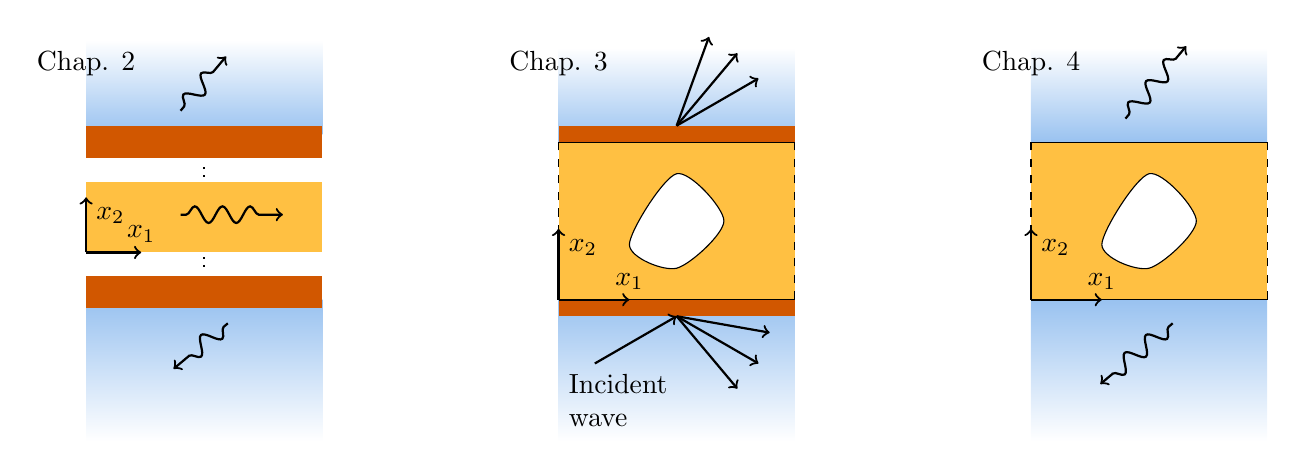
\begin{tikzpicture}
    \def\len{3}
    \def\height{1.5}
    \def\chapwidth{6cm}
     \def\pad{.3} 
    % CHAPTER 2
    \begin{scope}       
    \def\arrow{.7}
        \draw[top color = white, bottom color=fluid, draw=none] (0, \height+2*\pad) rectangle ++ (\len, 4*\pad);
        \draw[top color = fluid, bottom color = white,draw=none] (0, 0) rectangle ++ (\len, -6*\pad);
        \draw[fill=pem, draw=none] (0, 2*\pad) rectangle ++ (\len, \height-2*\pad);
        \draw[thick, dotted] (\len/2, \height+.2*\pad) -- ++ (0, .5*\pad);
        \draw[thick, dotted] (\len/2, 2*\pad-.2*\pad) -- ++ (0, -.5*\pad);
        \draw[fill=rubber, draw=none] (0, \height+\pad) rectangle ++ (\len, .4);
        \draw[fill=rubber, draw=none] (0, \pad) rectangle ++ (\len, -.4);
            \draw[thick,->] (0,2*\pad) -- ++ (\arrow, 0) node[above] {$x_1$};
    \draw[thick, ->] (0,2*\pad) -- ++ (0, \arrow) node[below right] {$x_2$};
    \draw[->,thick,decorate,decoration={snake,amplitude=3pt,pre length=2pt,post length=3pt}] (\len/2-\pad, \height+3*\pad) -- ++ (50:3*\pad) node[right] {};
    \draw[->,thick, decorate,decoration={snake,amplitude=3pt,pre length=2pt,post length=3pt}] (\len/2+\pad, -\pad) -- ++ (220:3*\pad) node[right] {};
        \draw[->,thick, decorate,decoration={snake,amplitude=3pt,pre length=2pt,post length=4pt}] (\len/2-\pad, \height-1.4*\pad) -- ++ (1.3, 0) node[right] {};
        \node at (0, 3) {Chap. 2};
    \end{scope}    
    % CHAPTER 3
    \begin{scope}[xshift=\chapwidth]   
    \def\cellen{\len} \def\height{2}\def\arrow{.9}\def\totalen{\cellen}
    \def\rubberthick{.7*\pad}
    \draw[top color = white, bottom color=fluid, draw=none] (0, \height) rectangle ++ (\totalen, 4*\pad);
    \draw[top color = fluid, bottom color = white,draw=none] (0, 0) rectangle ++ (\totalen, -6*\pad);
    \draw[fill=pem, draw=none] (0, 0) rectangle ++ (\totalen, \height);
    \draw[fill=rubber, draw=none] (0, \height) rectangle ++ (\totalen, \rubberthick);
    \draw[fill=rubber, draw=none] (0, 0) rectangle ++ (\totalen, -\rubberthick);

    \draw[black] (0, 0) -- ++ (\totalen, 0);
    \draw[black] (0, \height) -- ++ (\totalen, 0);
    \foreach \i in {0} {
            \draw[fill=white] plot[smooth cycle] coordinates {
            (\i*\cellen + \cellen/2, \height/2-2*\pad) 
            (\i*\cellen + \cellen/2 - 2*\pad, \height/2-\pad)
            % (\i*\cellen + \cellen/2-1.3*\pad, \height/2)
            (\i*\cellen + \cellen/2, \height/2+2*\pad)
            (\i*\cellen + \cellen/2 + 2*\pad, \height/2)
        };        
        \draw[dashed] (\i*\cellen, 0) -- ++ (0, \height);
        \draw[dashed] (\i*\cellen+\cellen, 0) -- ++ (0, \height);
        }
        
    \draw[thick,->] (0, 0) -- ++ (\arrow, 0) node[above] {$x_1$};
    \draw[thick, ->] (0, 0) -- ++ (0, \arrow) node[below right] {$x_2$};

    \draw[thick, ->] (\cellen/2, \height+\rubberthick) -- ++ (50:4*\pad) node[right] {};
    \draw[thick, ->] (\cellen/2, \height+\rubberthick) -- ++ (30:4*\pad) node[right] {};
    \draw[thick, ->] (\cellen/2, \height+\rubberthick) -- ++ (70:4*\pad) node[right] {};
    \draw[thick, <-] (\cellen/2, -\rubberthick) -- ++ (210:4*\pad)  node[below, xshift=12pt, text width=1.5cm] {Incident wave};
    \draw[thick, ->] (\cellen/2, -\rubberthick) -- ++ (-30:4*\pad) node[right] {};
    \draw[thick, ->] (\cellen/2, -\rubberthick) -- ++ (-50:4*\pad);
    \draw[thick, ->] (\cellen/2, -\rubberthick) -- ++ (-10:4*\pad);
    % \draw[dashed]    (\cellen/2, -\rubberthick) -- ++ (0, -4*\pad);

    \node at (0, 3) {Chap. 3};

\end{scope}  
%     % CHAPTER 4
    \begin{scope}[xshift=2*\chapwidth]   
\def\cellen{\len} \def\height{2}\def\arrow{.9}\def\totalen{\cellen}
    \def\rubberthick{.7*\pad}
    \draw[top color = white, bottom color=fluid, draw=none] (0, \height) rectangle ++ (\totalen, 4*\pad);
    \draw[top color = fluid, bottom color = white,draw=none] (0, 0) rectangle ++ (\totalen, -6*\pad);
    \draw[fill=pem, draw=none] (0, 0) rectangle ++ (\totalen, \height);

    \draw[black] (0, 0) -- ++ (\totalen, 0);
    \draw[black] (0, \height) -- ++ (\totalen, 0);
    \foreach \i in {0} {
            \draw[fill=white] plot[smooth cycle] coordinates {
            (\i*\cellen + \cellen/2, \height/2-2*\pad) 
            (\i*\cellen + \cellen/2 - 2*\pad, \height/2-\pad)
            % (\i*\cellen + \cellen/2-1.3*\pad, \height/2)
            (\i*\cellen + \cellen/2, \height/2+2*\pad)
            (\i*\cellen + \cellen/2 + 2*\pad, \height/2)
        };        
        \draw[dashed] (\i*\cellen, 0) -- ++ (0, \height);
        \draw[dashed] (\i*\cellen+\cellen, 0) -- ++ (0, \height);
        }
        
    \draw[thick,->] (0, 0) -- ++ (\arrow, 0) node[above] {$x_1$};
    \draw[thick, ->] (0, 0) -- ++ (0, \arrow) node[below right] {$x_2$};

    \draw[->,thick,decorate,decoration={snake,amplitude=3pt,pre length=2pt,post length=3pt}] (\cellen/2-\pad, \height+\pad) -- ++ (50:4*\pad) node[right] {};
    \draw[->,thick, decorate,decoration={snake,amplitude=3pt,pre length=2pt,post length=3pt}] (\cellen/2+\pad, -\pad) -- ++ (220:4*\pad) node[right] {};
    \node at (0, 3) {Chap. 4};
    \end{scope}  
\end{tikzpicture}
    \caption{Diagram presenting the various configurations studied in this work}
    \label{fig:intro_diagram}
\end{figure}

\begin{itemize}
    \item \textsc{Chapter} 1 introduces the fundamental concepts necessary for the good understanding of the thesis. This chapter focuses on the scattering of waves on dissipative layers and the guided waves formalism that is used for the calculation of dispersion relations. Additional bibliography is proposed on these topics as well as a summary of usable numerical methods to compute such problems.  
    \item \textsc{Chapter} 2 targets the study of the propagation of guided waves in multilayer arbitrary structures with dissipative layers. A simple numerical method, the \acrfull{scm} is implemented and extra steps allow for the local coupling of surrounding media allows for the computation of the dispersion relation for these configurations. This chapter is constituted from paper~\cite{marechal2025}. 

    \item \textsc{Chapter} 3 is focused on several numerical strategies for the modelling of scattering properties of metaporous/metaporoelastic structures. A global method is coupled to a \acrshort{fem}. Results focused on the performance of the proposed method, compared to other similar frameworks is proposed. The convergence of this method is shown for various metaporoelastic surfaces, which geometries were studied in previous papers. This chapter is originally an article referenced as paper.~\comment{cite this when finished}.
    \item In \textsc{Chapter} 4, the modal behaviour of metaporous structure is studied. The fem method from the previous chapter is adapted to describe this problem. Results are presented for the case of a rigid inclusion, as well as with embedded \acrfull{srr}. Contents for this chapter were published in paper.~\comment{cite this when finished}.
\end{itemize}

Finally, a summary of this work is proposed along with some perspectives on this work, including early results generalizing results from chapter four to include poroelastic hosts. 
\endgroup